%\documentclass{article}
%%\usepackage[english]{babel}%
%\usepackage{graphicx}
%\usepackage{tabulary}
%\usepackage{tabularx}
%\usepackage[table,xcdraw]{xcolor}
%\usepackage{pdflscape}
%\usepackage{lastpage}
%\usepackage{multirow}
%\usepackage{afterpage}
%\usepackage{rotating}
%\usepackage{pdfpages}
%\usepackage{cancel}
%\usepackage{amsmath}
%\usepackage[table]{xcolor}
%\usepackage{caption}
%\captionsetup{font=scriptsize,labelfont=scriptsize}
%\usepackage{pdflscape}
%\usepackage{fixltx2e}
%\usepackage[T1]{fontenc}
%\usepackage[utf8]{inputenc}
%\usepackage{multirow}
%\usepackage{ifthen}
%\usepackage{fancyhdr}
%\usepackage[document]{ragged2e}
%\usepackage[margin=1in,top=1.2in,headheight=57pt,headsep=0.1in]
%{geometry}
%\usepackage{ifthen}
%\usepackage{fancyhdr}
%\everymath{\displaystyle}
%\usepackage[document]{ragged2e}
%\usepackage{fancyhdr}
%\usepackage[table,xcdraw]{xcolor}
%% If you use beamer only pass "xcolor=table" option, i.e. \documentclass[xcolor=table]{beamer}
%\usepackage[normalem]{ulem}
%\useunder{\uline}{\ul}{}
%\everymath{\displaystyle}
%\linespread{2}%controls the spacing between lines. Bigger fractions means crowded lines%
%%\pagestyle{fancy}
%%\usepackage[margin=1 in, top=1in, includefoot]{geometry}
%%\everymath{\displaystyle}
%\linespread{1.3}%controls the spacing between lines. Bigger fractions means crowded lines%
%%\pagestyle{fancy}
%\pagestyle{fancy}
%\setlength{\headheight}{56.2pt}
%
%
%\chead{\ifthenelse{\value{page}=1}{\includegraphics[scale=0.3]{BassettCTCLogo}\\ \textbf \textbf Water - General Introduction}}
%\rhead{\ifthenelse{\value{page}=1}{Shabbir Basrai}{Shabbir Basrai}}
%\lhead{\ifthenelse{\value{page}=1}{}{\textbf Water - General Introduction}}
%
%
%\cfoot{}
%\lfoot{Page \thepage\ of \pageref{LastPage}}
%\rfoot{}
%\renewcommand{\headrulewidth}{2pt}
%\renewcommand{\footrulewidth}{1pt}
%\newcommand{\comment}[1]{\hspace{0em}{\small\textit{#1}}\bigskip\par}
%\begin{document}


\chapterimage{WaterChapterImage1}
\chapter{Water - General Introduction}

\vspace{0.2cm}
\begin{center}
\textbf{\textit{“If there is magic on this planet, it is contained in water.”}}
\end{center}
\begin{flushright}
\textit{Loren Eiseley}
\end{flushright}
\vspace{0.2cm}


\begin{minipage}{.7\textwidth} 
\begin{itemize}
\item Its chemical formula, H$_2$O, indicates that each of its molecules contains one oxygen and two hydrogen atoms, connected by covalent bonds. The hydrogen atoms are attached to the oxygen atom at an angle of 104.45\si{\degree}
\end{itemize}.
    \end{minipage}%
        \begin{minipage}{0.3\textwidth}
        \centering
        \includegraphics[scale=0.4]{Waterpolarity}
    \end{minipage}\\
\vspace{0.5cm}
\begin{itemize}
\item Unique properties of water arise from the shape of its molecule which is comprised of a much larger oxygen atom and two smaller hydrogen atoms.  Even though the water molecule is overall neutral, its bent shape results in the accumulation of positive charge near the oxygen end and negative charge near the hydrogen.  This differential in charges makes the water molecule polar. 

\item The constituents, size and polarity of the water molecule imparts unique properties which makes water vital not only for the existence of all biological lifeforms and for other non-biological aspects critical for the survival and progress of the human race.

\item Water makes up 60-75\% of human body weight. A loss of just 4\% of total body water leads to dehydration, and a loss of 15\% can be fatal. A person could survive a month without food but wouldn’t survive 3 days without water.\\
\end{itemize}

\subsection{Water use}\index{Water use}
\begin{itemize}
\item Besides it being needed for basic sustenance of all living beings, water is vital element for the world economy and sustenance of the human society in various ways including:
\begin{itemize}
\item As a food source - fishing
\item For commerce - shipping, trade and transportation
\item For recreation - swimming, skiing, surfing etc.
\end{itemize}
\item Breakdown of global freshwater use:\\
70\% is used for agriculture\\
19\% is used by industries, and \\
11\% is for municipal use

\item In the USA, average water consumption per person is about 80-100 gallons per day.

\end{itemize}

\section{Water Supplies}\index{Water Supplies}
\begin{itemize}
\item The water on our Earth today is the same water that has been here for nearly 5 billion years.\\
\item Water molecules were formed in interstellar space by chemical reactions between hydrogen molecules and oxygen-bearing molecules such as carbon monoxide and the Earth inherited its water from asteroids and comets crashing into it.
\item The only thing that changes is the form that water takes as it travels through the water cycle.
\item On Earth, water is the only substance that can occur naturally in its three states of matter -  gas, liquid and solids, circulates naturally through its five principal realms:
\begin{itemize}
\item Oceans
\item Atmosphere
\item Lakes and rivers
\item Icecaps and glaciers
\item Underground
\end{itemize}
This is the planetary Water Cycle.
\item Life on earth is dependent on the Earth's water cycle
\item Civilizations have always formed near water sources - on the banks of rivers. Ancient Egyptians - on the Nile, Mesopotamians in the Fertile Crescent on the Tigris/Euphrates rivers, Ancient Chinese on the Yellow River, and the Ancient India on the Indus.
\newpage
\begin{figure}[]
\begin{center}
\includegraphics[scale=0.8]{Watercycle1}
\caption{Water Cycle}
\textit{(Credit:David Cain/NWS)}
\end{center}
\end{figure}
\item Water covers about 71\% of Earth's surface.  The distribution of Earth's water is provided in the below table.

% Please add the following required packages to your document preamble:
% \usepackage{multirow}
\begin{table}[ht]
\begin{center}
\begin{tabular}{|l|l|llll}
\hline
\multirow{9}{*}{Fresh water} & \multirow{9}{*}{2.50\%} & \multicolumn{1}{l|}{\multirow{7}{*}{Surface water}} & \multicolumn{1}{l|}{\multirow{7}{*}{1.20\%}} & \multicolumn{1}{l|}{Atmosphere}                & \multicolumn{1}{l|}{3.00\%}  \\ \cline{5-6} 
                             &                         & \multicolumn{1}{l|}{}                               & \multicolumn{1}{l|}{}                        & \multicolumn{1}{l|}{Living things}             & \multicolumn{1}{l|}{0.26\%}  \\ \cline{5-6} 
                             &                         & \multicolumn{1}{l|}{}                               & \multicolumn{1}{l|}{}                        & \multicolumn{1}{l|}{Rivers}                    & \multicolumn{1}{l|}{0.49\%}  \\ \cline{5-6} 
                             &                         & \multicolumn{1}{l|}{}                               & \multicolumn{1}{l|}{}                        & \multicolumn{1}{l|}{Swamps, marshes}           & \multicolumn{1}{l|}{2.60\%}  \\ \cline{5-6} 
                             &                         & \multicolumn{1}{l|}{}                               & \multicolumn{1}{l|}{}                        & \multicolumn{1}{l|}{Soil moisture}             & \multicolumn{1}{l|}{3.80\%}  \\ \cline{5-6} 
                             &                         & \multicolumn{1}{l|}{}                               & \multicolumn{1}{l|}{}                        & \multicolumn{1}{l|}{Lakes}                     & \multicolumn{1}{l|}{20.90\%} \\ \cline{5-6} 
                             &                         & \multicolumn{1}{l|}{}                               & \multicolumn{1}{l|}{}                        & \multicolumn{1}{l|}{Ground ice and permafrost} & \multicolumn{1}{l|}{69.00\%} \\ \cline{3-6} 
                             &                         & \multicolumn{1}{l|}{Ground water}                   & \multicolumn{1}{l|}{30.10\%}                 &                                                &                              \\ \cline{3-4}
                             &                         & \multicolumn{1}{l|}{Glaciers and ice caps}          & \multicolumn{1}{l|}{68.70\%}                 &                                                &                              \\ \cline{1-4}
Other saline   water         & 0.90\%                  &                                                     &                                              &                                                &                              \\ \cline{1-2}
Oceans                       & 96.50\%                 &                                                     &                                              &                                                &                              \\ \cline{1-2}
\end{tabular}
\caption{Distribution of Earth's Water}
\textit{(From:  Igor Shiklomanov's chapter "Worlds fresh water resources" in Peter H. Gleick (editor), \\1993, Water in Crisis: A guide to the world's Fresh water resources)}
\end{center}
\end{table}
\item 97\% of the Earth's water can be found in our ocean and freshwater is only 2.5\% of all the water on earth
\item Most of the fresh water is in form of ice in glaciers, ice caps and permafrost.  
\item A very very small fraction - about 0.006\% of the total water is the freshwater in lakes and rivers.  Most of the remaining freshwater is in groundwater - about 0.75\% of the total water or about 30\% of the total freshwater.
\item Source water refers to bodies of water (such as rivers, streams, lakes, reservoirs, springs, and ground water) that provide water to public drinking-water supplies and private wells. Water sources can include:

\begin{itemize}
\item Surface water (for example, a lake, river, or reservoir)
\item Ground water (for example, an aquifer)
While the volume of groundwater in California is very large, aquifers can be over drafted when groundwater is removed more rapidly than it is replenished.
\item Recycled water external icon (also called reused water)\\
\end{itemize}




\item Within the Water Cycle, there are many subcycles which can be regional or local.
\item One such cycle is the local cycle which involves water use and reuse.\\

\begin{figure}
\includegraphics[scale=0.2]{Test4}\\
\captionof{figure}{Water Use - Reuse Cycle}%\caption{}
\end{figure}

\item Water reuse (also commonly known as water recycling or water reclamation) reclaims water from a variety of sources then treats and reuses it for beneficial purposes such as agriculture and irrigation, potable water supplies, groundwater replenishment, industrial processes, and environmental restoration.
\item Water reuse can provide alternatives to existing water supplies and be used to enhance water security, sustainability, and resilience.

\item Unplanned or de facto reuse refers to situations in which a source of water is substantially composed of previously-used water. An example of unplanned water reuse occurs when communities draw their water supplies from rivers, such as the Colorado River and the Mississippi River, that receive treated wastewater discharges from communities upstream.



\item Clean water is vital to our health, communities, and economy. 
\item There is no universally accepted definition of “safe drinking water.” Generally speaking, safe drinking water, is defined as the water that does not represent any significant risk to health over a lifetime of consumption.
\item The water cycle is primarily water exchange between the ocean and atmosphere
\item The amount of water that is available for use is only a very small fraction of the total amount of water in existence.
\item Water scarcity can be caused by a mix of hydrological, infrastructural, political and social issues. 
\item In developing countries, water supply and sanitation related factors cause more than 20 percent of deaths of people under age 14. Nearly
half of all people in developing countries have infections or diseases associated with inadequate water supply and sanitation.
\item Chemical contaminants in drinking water arise including arsenic, fluoride or nitrate, emerging contaminants such as pharmaceuticals, pesticides, per- and polyfluoroalkyl substances (PFASs) and microplastics generate public concern.
\item Microbiologically contaminated drinking water can transmit diseases such as diarrhoea, cholera, dysentery, typhoid and polio and is estimated to cause 485 000 diarrhoeal deaths each year.
\item The amount of water that is available for sustenance including agriculture, sanitation and hygiene is limited in many areas of the world.  Billions of people throughout the world are battling daily against enormous difficulties accessing the most basic services.\\
\item Some 1.1 billion people worldwide lack access to water, and a total of 2.7 billion find water scarce for at least one month of the year.
\item Inadequate sanitation is also a problem for 2.4 billion people—they are exposed to diseases, such as cholera and typhoid fever, and other water-borne illnesses. Two million people, mostly children, die each year from diarrheal diseases alone.\\
\item Many of the water systems that keep ecosystems thriving and feed a growing human population have become stressed. Rivers, lakes and aquifers are drying up or becoming too polluted to use. More than half the world’s wetlands have disappeared.
\item Climate change is altering patterns of weather and water around the world, causing shortages and droughts in some areas and floods in others, changing large-scale hydrological cycle.\\
\item At the current consumption rate, this situation will only get worse. By 2025, two-thirds of the world’s population may face water shortages. And ecosystems around the world will suffer even more\\
\item Factors affecting water supplies include:
\begin{enumerate}
\item Pollution\\
Surface waters - streams, rivers, lakes which may be the source of drinking water supply are easily contaminated by agricultural and urban runoffs with fertilizer, pesticides, oil, dirt, bacteria and other pollutants.\\
\vspace{0.2cm}
Even groundwater is not safe from pollution, as many pollutants can leach into underground aquifers. Some effects are immediate, as when harmful bacteria from human waste contaminate water and make it unfit to drink or swim in.\\
\vspace{0.2cm}
Even trace levels of heavy metals, dyes, and microbes are hazardous to human health, aquatic systems, and the environment.\\
\vspace{0.2cm}
In other instances—such as toxic substances from industrial processes—it may take years to build up in the environment and food chain before their effects are fully recognized.\\
\begin{figure}[htp]
\begin{center}
%\includegraphics[landscape=true]{Test4.pdf}
\includegraphics{WaterContamination}\\
\captionof{figure}{Water Contamination}
\end{center}
\end{figure}


\item The state’s water supplies are from surface water sources such as rivers, streams, and lakes and from groundwater sources, which are present in groundwater basins throughout the state. The amount of drinking water derived from surface water sources versus groundwater sources can vary annually depending on rainfall and snowpack conditions. In general, surface water sources provide a larger portion of the drinking water supply than
\item groundwater sources; however, 90 percent of the public water systems only have groundwater. For example, the United States Geological Survey (USGS) estimated that, in 2015 in California, 54 percent of the drinking water provided by public water systems was from surface water sources (https://pubs.er.usgs.gov/publication/cir1441). This is down dramatically from the 2010 report, were it was over 80 percent of the state’s drinking water was from surface water sources. This change may be due to drought conditions, which significantly increases reliance on groundwater sources. Table 3-1 shows over 90 percent of the source drinking water facilities are groundwater wells.
\item As most of the surface water sources are already allocated, additional water needs have been met through groundwater sources. Historically, the use of groundwater was not regulated. As demand for groundwater continued to increase, effective management was needed to protect the future availability and quality of the supply. In September 2014, Governor Edmund G. Brown Jr. signed a three-bill package known as the Sustainable Groundwater Management Act (SGMA). The legislation allows local agencies to adapt groundwater sustainability plans to their regional economic and environmental needs. The Act creates a framework for sustainable, local groundwater management for the first time in California history. The primary responsibility assigned to the State Water Board is to protect groundwater resources if a local agency cannot or will not manage its groundwater sustainably. If local efforts fail to adequately manage groundwater, the State Water Board has the authority to step in and collect groundwater data, designate the basin as probationary, develop groundwater management plans, and collect fees for these activities. 
\item Over-extraction of groundwater to meet community and agricultural needs, particularly during times of drought, can reduce the availability of this important source of drinking water. Monthly monitoring of both the static and pumping water levels will provide information on the effects of drought-related and overdrafting stresses on groundwater sources. The California Water Plan Update 2018 points out the significance of groundwater withdrawal, particularly to the Central Valley, where most of California’s groundwater extraction occurs (https://water.ca.gov/Programs/California-Water- Plan/Update-2018).
The loss of groundwater can lead to increased pumping costs to access water from greater soil depths. In addition, groundwater loss from its aquifers can result in land subsidence, which can damage water-related infrastructure such as canals, resulting in water loss. The associated collapse of the hydrogeological structure of aquifers is problematic for their ability to rehydrate, and can interfere with the functionality of drinking water wells. A 2019 DWR press release on subsidence in the Sacramento Valley presents an example of the problems that subsidence presents
\item Alternative or Supplemental Sources of Drinking Water
In addition to the usual surface and groundwater sources of drinking water, there are alternative or supplemental sources of water, which may be used to augment drinking water supplies. These include recycled water and desalination, which may be used to treat seawater or brackish groundwater.
\begin{itemize}
\item Recycled Water\\
There has been considerable development in the use of recycled water to supplement drinking water supplies. Recycled water is obtained from municipal wastewater (sewage)
treatment plants and is treated prior to its reuse. It is likely that recycled water will become a more significant source of drinking water in some areas of California.
Recycled water may be used as an indirect source of drinking water (called indirect potable reuse), wherein recycled water is used to augment groundwater or surface water sources, by being introduced into those sources after additional treatment and prior to further treatment before it is made available for consumption by drinking water customers.
Most of the indirect potable reuse water activity to date has been in Orange County, in San Bernardino County, and in Los Angeles County, where recycled water has been highly treated and reintroduced to groundwater by direct injection or by the use of recharge basins, from which the recycled water percolates into underground aquifers. New projects are also planned in Monterey County. In addition, the City of San Diego is planning a surface water augmentation project. San Diego has extensively studied the use of highly treated recycled water to supplement its surface water drinking water supplies.
Indirect potable reuse projects operate under permits issued by the Regional Water Boards, who consult with DDW to establish conditions necessary to protect drinking water supplies. In addition, the State Water Board now has authority to issue indirect potable reuse permits.
To assist in the development of recycled water projects for groundwater replenishment that are protective of public health, regulations for such projects were adopted and became effective on June 18, 2014.
Since the 2015 Plan, as required by Chapter 700, Statutes of 2010 (SB 918), the State Water Board adopted regulations for surface water augmentation in December 2016. These regulations were developed following the findings of the Expert Panel formed pursuant to SB 918 that such regulations would be protective of public health for this use. The regulations are found at the DDW website mentioned above.
Recycled water is also being considered as a direct source of drinking water, which would be introduced directly into a public water system’s distribution system for customer use (direct potable reuse). Under SB 918 and SB 322 (Chapter 637, Statutes of 2013), the State Water Board was required to investigate and report on the feasibility of developing uniform water recycling criteria for direct potable reuse. A report to the legislature was submitted in December 2016; it concluded that the development of such criteria was feasible, but that there were significant data gaps and research needs to ensure adequate public health protection.
Use of alternative water supplies such as indirect potable reuse for groundwater replenishment and surface water augmentation for drinking water requires considerable treatment to provide adequate public health protection. Care must be taken to ensure the required high level of water treatment does not fail, so customers do not receive unsafe
drinking water. For direct potable reuse projects, where the connection between highly treated wastewater and treated drinking water is more proximal and immediate than it is in indirect potable reuse projects, more treatment and highly focused operations will be required for the protection of public health.
The purpose of current and potential future State Water Board water recycling regulations is to ensure that project design, construction, and operation are protective of public health. \\
In 2019, the State Water Board completed a revision to the Framework (Framework Second Edition) to reflect the State Water Board’s current thinking on regulating direct potable reuse. The Framework Second Edition includes a discussion of the regulatory approach for direct potable reuse, as well as an update on the consideration of drinking water treatment plants. The Framework Second Edition is presented in a format that highlights the revisions that were made.
\item Desalination
Desalination of water that is otherwise not fit for consumption may provide another source of supplemental water supply. Typically, desalination is either categorized as seawater or brackish water desalination. Seawater desalination treats ocean water obtained from either an open water intake or a subsurface intake to a treatment plant is located near the coast, Brackish water desalination treats groundwater with elevated salt levels and can occur in both inland and coastal areas.
There are four seawater desalination facilities in California that produce drinking water. The permitted seawater desalination facilities are shown in Table 3-2. Other coastal counties have proposed desalination facilities but have not yet begun construction.
\end{itemize}

\begin{table}[]
\begin{tabular}{|l|l|l|}
\hline
Desalination   Project                                   & Production                                 & County   Served           \\ \hline
Claude   "Bud"   Lewis   Carlsbad   Desalination   Plant & 56,000   acre-ft   per   year   (50   MGD) & San   Diego               \\ \hline
Charles   E.   Meyer   Desalination   Plant              & 3,125   acre-ft   per   year   (2.8 MGD)   & Santa   Barbara           \\ \hline
Santa   Catalina   Island   Desalination   Plant         & 364   acre-ft   per   year   (0.33   MGD)  & Santa   Catalina   Island \\ \hline
Sand   City   Coastal Desalination   Plant               & 336   acre-ft   per   year   (0.30   MGD)  & Monterey                  \\ \hline
\end{tabular}
\caption{Permitted De-Salination Facilities in California}
\end{table}



\begin{table}[]
\begin{tabular}{|l|l|}
\hline
Water   Source                                                  & Number   of   Facilities \\ \hline
Surface   Water                                                 & 939                      \\ \hline
Groundwater   under   direct   influence   of   surface   water & 281                      \\ \hline
Groundwater                                                     & 15,041                   \\ \hline
\end{tabular}
\caption{Water System Facilities (2020 Data)}
\end{table}



\item Water supply diversion for agriculture and energy production\\
Agriculture uses 70\% of the world’s accessible freshwater.  Water diversions for agriculture usage, for supplying urban populations and for energy generations have significantly affected local water supplies both for human consumption and for sustaining the natural habitat and ecosystems.

\item Population growth\\
In the last 50 years, the human population has more than doubled. This rapid growth — with its accompanying economic development and industrialization—has transformed water ecosystems around the world and resulted in a massive loss of biodiversity.
\vspace{0.2cm}
The population increase exercises Concern about water availability grows as freshwater use continues at unsustainable levels. Furthermore, these new faces also need food, shelter, and clothing, thus resulting in additional pressure on freshwater through the production of commodities and energy.\\

\item Climate change\\
Climate change increases the odds of worsening drought in many parts of the world. In many places, droughts are expected to get more frequent, intense, and longer lasting.\\

How climate change contributes to drought:\\

\begin{itemize}
\item Warmer temperatures enhance evaporation, making periods with low precipitation drier than they would be in cooler conditions.
\item Climate change alters the timing of water availability. Warmer winter temperatures are causing less precipitation to fall as snow resulting in a decreased snowpack which:
\item Impact water management systems which rely on spring snowpack melt
\item Impact certain ecosystems which depend on snow melt to supply cold water for species like salmon. 
\item Exacerbates drought because of because of increases surface temperatures caused by a decreased reflective surface of the snow.
\item Warming increases precipitation variability, meaning there will be more periods of both extreme precipitation and drought. This creates the need for expanded water storage during drought years and increased risk of flooding and dam failure during periods of extreme precipitation.\\
\end{itemize}
\end{enumerate}


\begin{figure}
\begin{center}
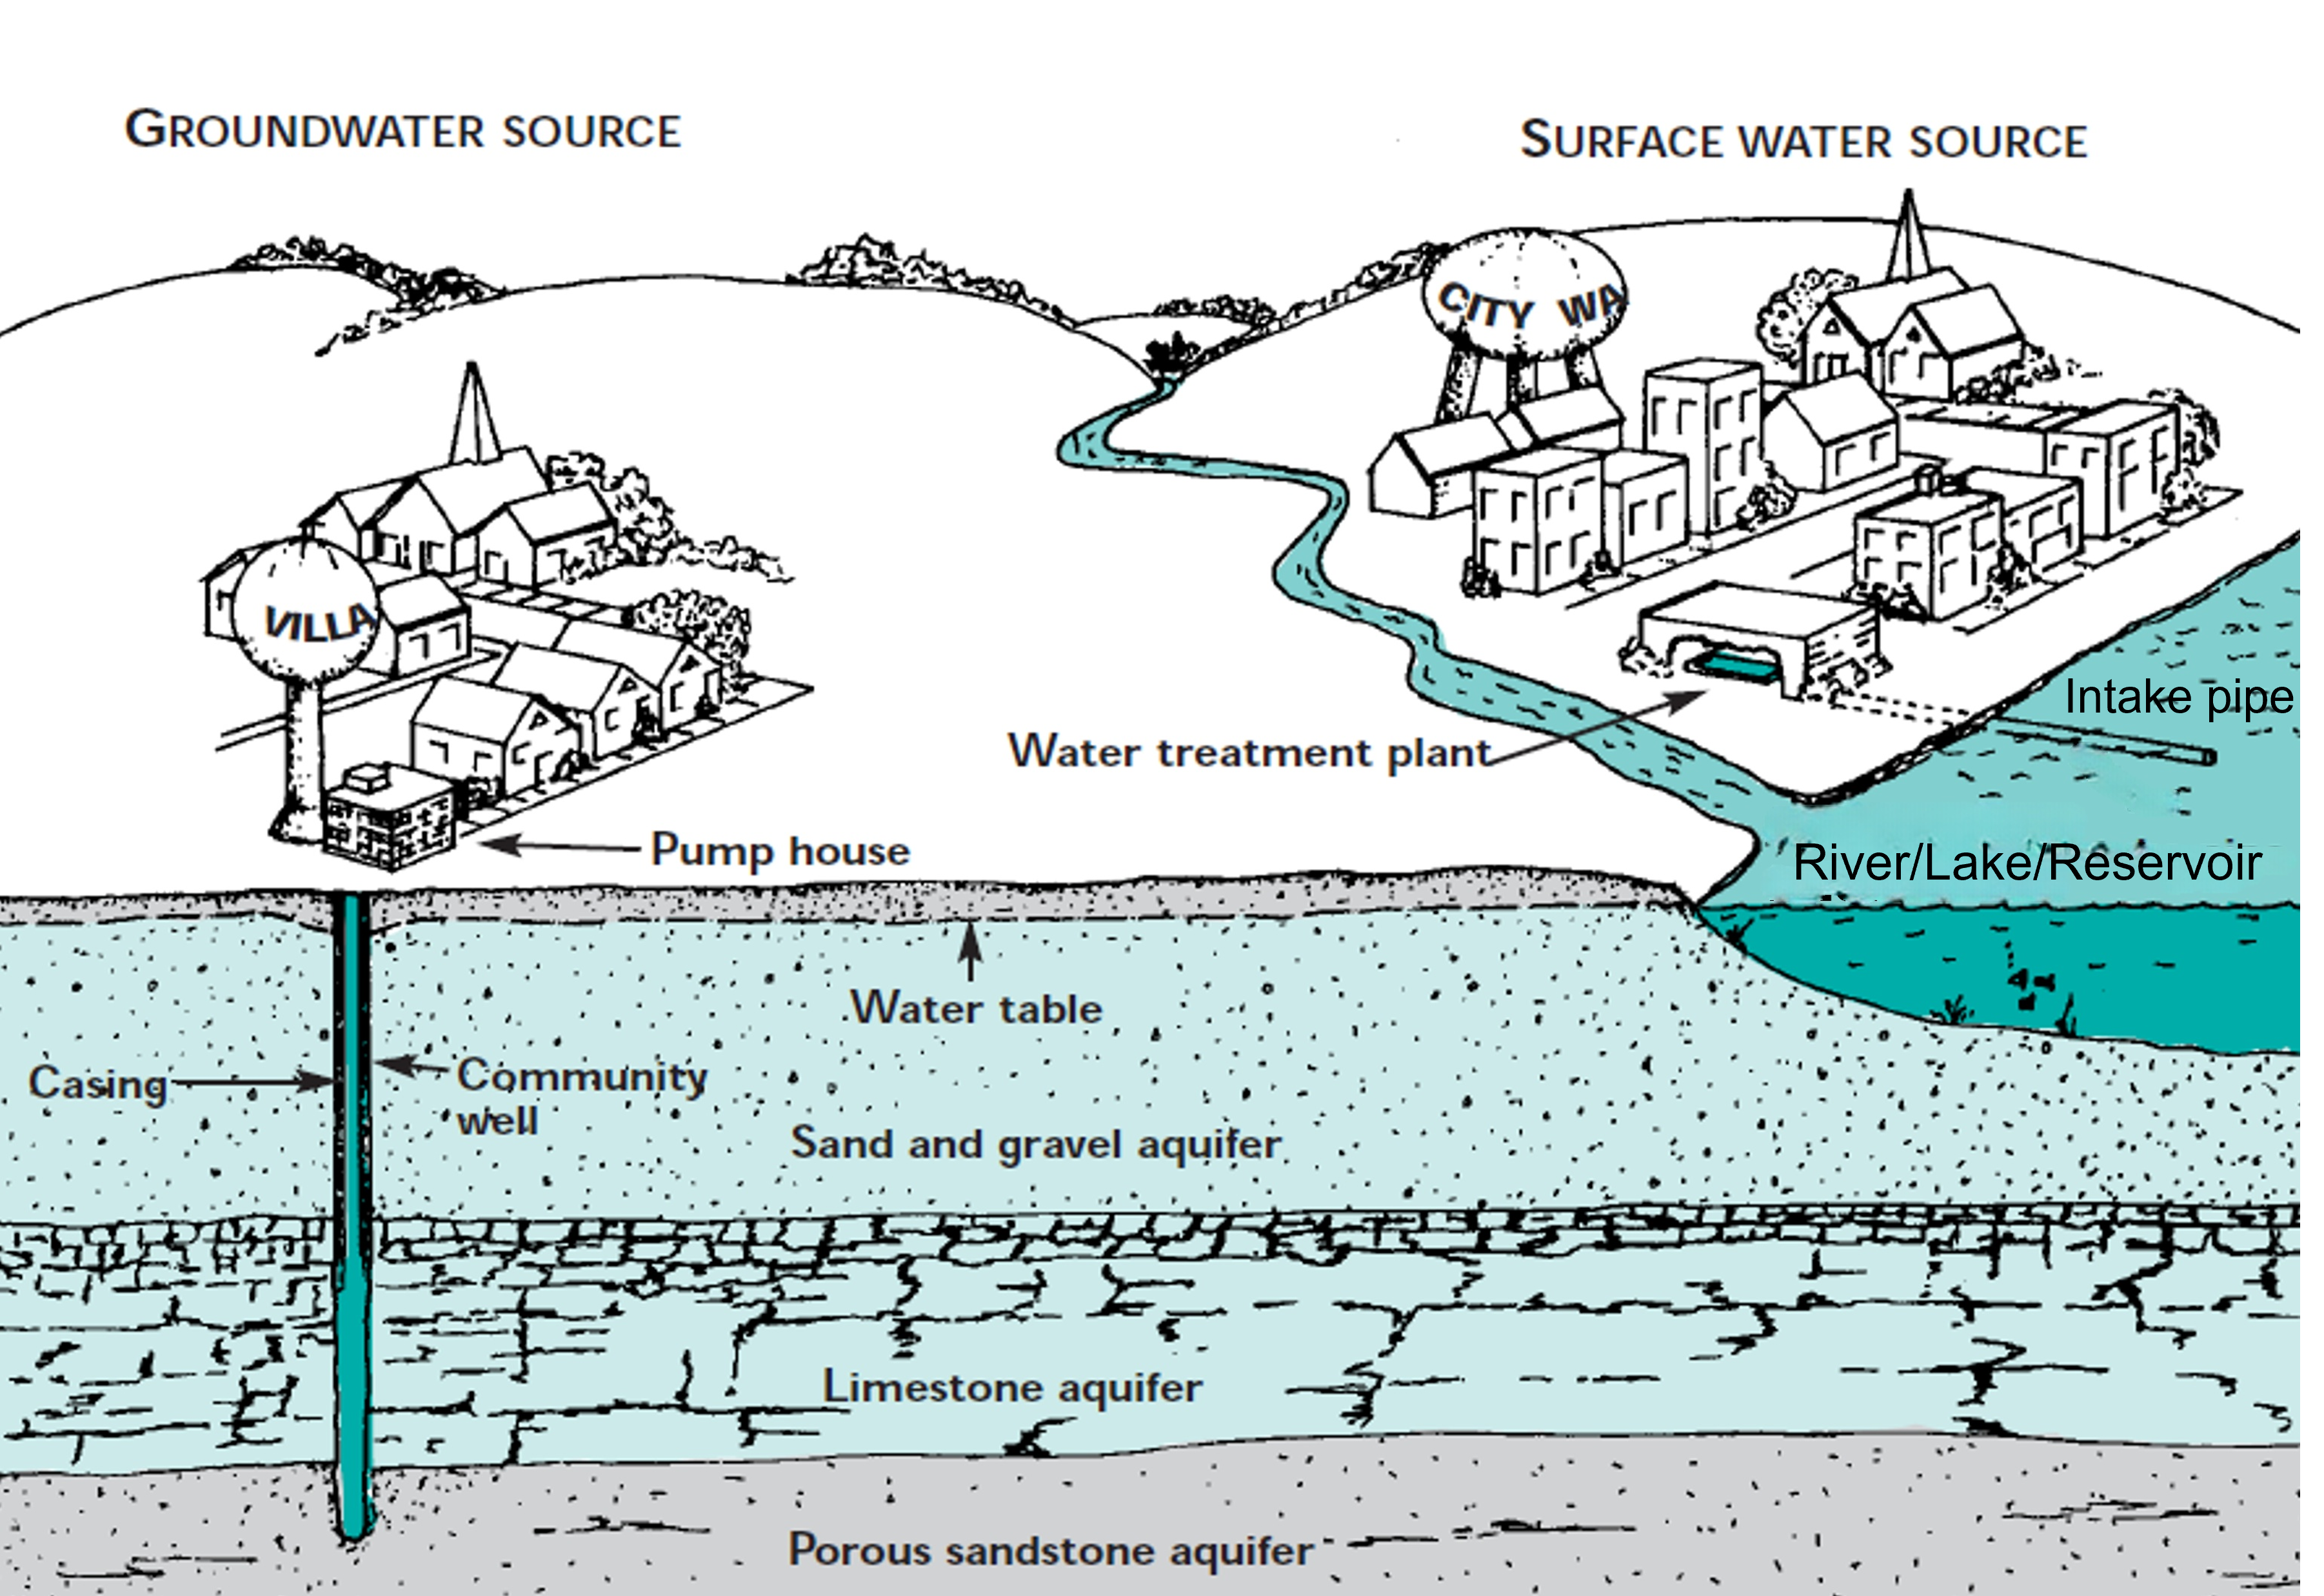
\includegraphics[scale=0.5]{WaterSources}\\
\captionof{figure}{Water Supply Sources}%\caption{}
\end{center}
\end{figure}
\begin{enumerate}
\item Groundwater
\begin{itemize}
\item Groundwater is considered to be water that is below the earth’s crust, but not more than 2500 feet below the crust. Water between the earth’s crust and the 2500-foot level is considered usable fresh water.\\

\item A watershed is an area of land that contributes water to a given location, such as a reservoir, a confluence of two streams, or the ocean. Within a watershed, water from rain or snow flows down the slope, through the soil, or via groundwater flow – and usually by a combination of these routes – to reach the stream and contribute to the flow of the stream. Watersheds are
important sources of drinking water, as well as a habitat for many aquatic species. Healthy watersheds with intact native vegetation and wetlands provide important functions such as water purification, flood control, nutrient recycling, and groundwater recharge.

\item An aquifer is a body of porous rock or sediment saturated with enough groundwater that it can be pumped to the surface and used for drinking water, irrigation, industry, or other uses. . Groundwater enters an aquifer as precipitation seeps through the soil. It can move through the aquifer and resurface through springs and wells.

\item Where groundwater can move rapidly, such as through gravel and sandy
deposits, an aquifer can form.  

\item There are two general types of aquifers: confined and unconfined. Confined aquifers have a layer of impenetrable rock or clay above them, while unconfined aquifers lie below a permeable layer of soil.

\item A common misconception about aquifers is that they are underground rivers or lakes. While groundwater can seep into or out of aquifers due to their porous nature, it cannot move fast enough to flow like a river. The rate at which groundwater moves through an aquifer varies depending on the rock’s permeability.

\item Much of the water we use for domestic, industrial, or agricultural purposes is groundwater. Most groundwater, including a significant amount of our drinking water, comes from aquifers. In order to access this water, a well must be created by drilling a hole that reaches the aquifer. While wells are manmade points of discharge for aquifers, they also discharge naturally at springs and in wetlands.

\item Groundwater can become depleted if we use it at a faster rate than it can replenish itself. The replenishment of aquifers by precipitation is called recharging. Depletion of aquifers has increased primarily due to expanding agricultural irrigation. Groundwater can become contaminated when an excessive amount of pesticides and herbicides are sprayed on agricultural fields, septic tanks leak, or landfills are improperly lined or managed and toxic materials seep through the soil into the aquifer.

\item Aquifers naturally filter groundwater by forcing it to pass through small pores and between sediments, which helps to remove substances from the water. This natural filtration process, however, may not be enough to remove all of the contaminants.

\item Groundwater is obtained from the following:\\
\begin{itemize}
\item Wells
\item Springs that are not influenced by surface water or a local hydrologic event
\item When a well or spring is influenced by an adjacent surface water source or by a local hydrological event, the supply is said to be groundwater under the direct influence of surface water (GUDISW).
\end{itemize}
\item Advantages of groundwater with respect to surface water:\\
\begin{itemize}
\item Groundwater is not as easily contaminated as surface water.
\item The quality of groundwater, while not always as good as would be preferred, is stable throughout the year.
\item Groundwater sources are generally lower in bacteriological count than surface water sources.
\item Groundwater is available in most locations throughout the continental US and Alaska.
\end{itemize}
\item Disdvantages of groundwater with respect to surface water:\\
\begin{itemize}
\item Once a groundwater source is contaminated, it is difficult for it to recover. There is no easy way to remove the contaminants.
\item Groundwater usually contains more minerals than surface water, including increased levels of hardness. Because groundwater is in contact longer with minerals, there is more time to bring them into solution.
\item Removal of groundwater normally requires a pump, thus increasing operation cost.
\item Groundwater is more susceptible to long-term contamination from fuel spills.
\item Groundwater supplies often have high levels of iron and manganese, thus increasing treatment cost and/or causing stains on plumbing and the clothing of customers.
\item Wells in the coastal areas are subject to salt water intrusion into the aquifer20
and well. This contamination is difficult to predict and costly to treat.
\item Sources of contamination can be hidden from sight.
\end{itemize}
\end{itemize}

\item Surface water\\
\begin{itemize}
\item Surface water is water that is open to the atmosphere and results from overland flow. It is also said to be the result of surface runoff 3. These are two ways of saying the same thing.
\item Examples of surface water include:
\begin{itemize}
\item Streams, Rivers, Lakes
\item Man-made impoundments - Reservoirs
\item Wells drilled next to or in a stream or river
\item Rain catchments
\end{itemize}

\item Advantages of surface water with respect to groundwater:
\begin{itemize}
\item It is easily located. It takes no sophisticated equipment to find a surface water source.
\item In many parts of the US, considerable data is available on quantity and quality of existing surface water supplies.
\item Surface water is generally softer than groundwater, which makes treatment much simpler.
\end{itemize}
\item Disadvantages of surface water with respect to groundwater:
\begin{itemize}
\item Surface waters can be easily contaminated with microorganisms that cause waterborne diseases and chemicals that enter the stream from surface runoff and upstream discharges.
\item The turbidity of a surface water source often fluctuates with the amount of precipitation. Increases in turbidity increase treatment cost and operator time.
\item The temperature of surface water fluctuates with the ambient temperature. This makes it difficult to produce consistent water quality at a water treatment plant.
\item The intake structure may become clogged or damaged from winter ice, or the source may be so shallow that it completely freezes in the winter. This is a common problem with surface water sources in the arctic.
\item Removing surface water from a river, lake, or reservoir requires a legal right, referred to as a water right. 
\item Using surface water as a source means that the purveyor is obligated to meet the requirements of the Surface Water Treatment Rule (SWTR) of the State Drinking Water Regulations. This rule requires that, in most instances, any surface water source must have a filtration system.
\item Surface waters that are high in color, especially color that is the result of decaying vegetation, have the potential to produce high levels of Total Trihalomethanes (TTHM). These chemical compounds are formed when chlorine is added to the water. The problem with the TTHM is that some of them are carcinogenic (can cause cancer) and are referred to as disinfection by-products (DBP).
\end{itemize}
\end{itemize}
\end{enumerate}

In the United States, 9 out of 10 people get their water from one of more than 148,000 public water systems. To make sure water from these systems is safe to drink, federal, state, and local authorities regulate and monitor public water systems.\\

\begin{figure}
\begin{center}
\includegraphics[scale=0.24]{waterSupplyIllustration1}\\
\captionof{figure}{Southern California Water Supply Illustration}%\caption{}
\end{center}
\end{figure}

\begin{figure}
\begin{center}
\includegraphics[scale=0.40]{LosAngelesWaterSupply}\\
\captionof{figure}{Los Angeles County Water Supply Sources}%\caption{}
\end{center}
\end{figure}

California primarily relies on a mixture of surface water and groundwater supplies for drinking water. The balance of supplies used in a given year is dependent upon the region of the state, water needs, water resource availability, and long-term weather conditions within the state. During periods of normal to high rainfall, surface water sources make up a higher percentage of the overall drinking water supplies across the state. However, use of groundwater increases and surface water supplies are strained during periods of lower than average rainfall.\\


The California State Water Project (SWP):\\

Managing water remains one of the great challenges for California. Population growth, a shifting climate, and declining ecosystem health are putting pressure on the state’s water supply and flood management systems.\\

 is a multi-purpose water storage and delivery system that extends more than 705 miles -- two-thirds the length of California. A collection of canals, pipelines, reservoirs, and hydroelectric power facilities delivers clean water to 27 million Californians, 750,000 acres of farmland, and businesses throughout our state.\\

 Such valuable
functions are sometimes referred to as “ecosystem services” (Revenga et al. 1998).\\
Californians rely on both surface and ground water sources for their domestic water supply. Unfortunately, the watersheds that yield water to these sources face many sources of degradation including sedimentation and pollution from residential and industrial development, timber harvests, agricultural production, land clearing, and mining (Revenga et al. 1998, Bolund and Hunhammar 1999). While these types of degradation can affect both surface
and groundwater, this report focuses on surface drinking water sources and watersheds. However, protecting and/or restoring native vegetation in these watersheds can also improve groundwater supply by maintaining or increasing groundwater recharge rates.\\
Mapping the watersheds that supply drinking water to people is a crucial first step to ensure they remain healthy and protected. Previous studies have listed sources or mapped a subset of the watersheds (e.g., the watersheds for one city), but none of these explicitly mapped all 
watersheds that supply drinking water to Californians1
\end{itemize}
\section{Cost of Water}\index{Cost of Water}
\begin{itemize}
\item Water costs have, on average over a five- year period from 2012 to 2017, increased about 35 percent within all size groups of water systems (range of 23 to 40 percent). \item Average water costs remain highest in the San Francisco Bay Area, Central Coast, and Southern California, and lowest in the Central Valley/Agricultural (including Imperial County), Foothill, and Mountain/Desert regions. 
\item On average, customers of small water systems (PWS serving fewer than
200 service connections) pay approximately 21 percent more for water than those customers served by larger systems.
\item Many economically disadvantaged communities are served by small water systems. As a result, water affordability has become a significant issue among residents in these communities.

\item Small water systems continue to have the largest percent of water quality problems and the highest rate of noncompliance with drinking water standards. In particular, small water systems serving between 15 and
200 service connections have the greatest noncompliance rates, especially those that serve disadvantaged communities.
Many of these small water systems lack the necessary resources to comply. 

\item There are more than 1,300 State Small water systems servicing about 32,000 people. Many of these systems are vulnerable to the same problems that small public water systems confront. However, State Small water system requirements are much less strict than those placed on PWS and those systems are not subject to addressing water quality problems unless they become PWS.

\end{itemize}

\section{Drinking Water Regulations}\index{Drinking Water Regulations}
\begin{itemize}
\item Timeline of key legislation on regulating water quality is given below.
\begin{enumerate}
\item 1893 – U.S. Public Health Service (USHPS) enacts Interstate Quarantine Act, a regulation prohibiting use of a common drinking cup by passengers on commercial transportation carriers traveling between states.
\item 1914 - Federal standard for bacteriological water quality developed.
\item USPHS expanded standards to include guidelines for bacteriological sampling and maximum levels for lead, fluoride, arsenic, selenium, and chromium. Generally, these were non-enforceable guidelines.
\item 1962 – Guidelines are expanded to include additional constituents. Limits on many constituents made mandatory.
\item 1974 – Congress passes Safe Drinking Water Act.
\item 1986 and 1996 - Safe Drinking Water Act amended.
\end{enumerate}

\item United States Environmental Protection Agency (EPA)  is mandated by Congress through the Safe Drinking Water Act to establish drinking water regulations and periodically review these regulations to update them.

\item EPA studies health issues related to water quality and develops regulations, standards, and guidance documents related to drinking water. It legislates specific minimum requirements that the states must meet, though the states are generally permitted to enact more stringent requirements.

\item The United States Environmental Protection Agency (EPA) defines a Public Water System as “a system for the provision to the public of water for human consumption through pipes or other constructed conveyances, if such system has at least fifteen service connections or regularly serves an average of at least twenty-five individuals daily at least 60 days out of the year.”

\item Each Public Water System is required to have domestic water supply permits and is responsible for providing affordable, safe drinking water to their customers 24 hours a day, 7 days a week, 365 day a year.

\item All public water systems are subject to the same health based standards and laws whether they are a big city, a small community, or a rural restaurant. However, there are some minor adjustments that are made to monitoring frequencies based on population and water system type.

\item Requirements of a Public Water Agency in California include:

\begin{itemize}

\item Permitting engineering and technical reports, including pump tests, at least two water supply well sources for communities, a 50-foot radius source protection zone around all new wells, a minimum of a 50-foot annular seal on new wells , a well flow meter and initial monitoring \\
\item  Construction, including elevated storage or backup electricity for pumps to maintain 40 pounds per square inch (psi) minimum pressure at all times, proper construction of distribution systems, adequate storage capacity and fire fighting capacity \\
\item  As-built maps.\\
\item  Annual water-treatment chemicals and equipment for distribution monitoring of any added chemical treatment (dependent on the type of needed treatment) \\
\item  Ongoing raw water chemical monitoring sampling and analysis. \\
\item  Ongoing raw water bacteriological monitoring sampling and analysis. \\
\item  Ongoing treated water bacteriological monitoring sampling and analysis.\\
\item  Maintenance of bacteriological plans and emergency notification plans for water quality emergencies . \\
\item  Ongoing lead and copper monitoring including sampling and analysis and maintenance of a lead and copper plan. \\
\item  Ongoing disinfection byproducts monitoring and maintenance of an associated plan.\\
\item  Maintaining a customer water quality complaint program.\\
\item  Main flushing, valve and meter maintenance, and maintaining system maps.\\
\item  Cross connection program and annual back-flow device testing.\\
\item  Licensed water treatment operator and distribution staff.\\
\item  Written procedures for system maintenance, for example pipeline break procedures, etc.\\
\item  Source capacity planning studies and permit amendments for any additional growth.\\
\item  Annual Consumer Confidence Report preparation and distribution. Requirements continue on next page.\\
\item  Annual Electronic Report submittal to State Water Resource Control Board-Division of Drinking Water \\
\item  Records of the estimated life of all pumps, treatment, storage, and distribution system and an annual capital improvement plan to fund infrastructure replacement.\\
\item  Metering and billing staff.\\
\item  Emergency reserves for drought, regulatory changes, public notice of bacteriological or chemical failures, etc. (CHSC §116540) \\
\item  Maintaining of business licenses, annual drinking water permit fees and payment of any State enforcement fees for actions resulting from water system non-compliance .\\
\item  Appropriate working area for staff, chemicals, and records \\
\item  Insurance and liability for staff, with duties including climbing tanks, handling hazardous chemicals, etc. \\
\item  Management staff that is knowledgeable about drinking water. Staff coordinate the above and maintain financial controls.\\
\item  If the source is surface water, there may be additional requirements: o A water treatment plant meeting all Surface Water Treatment Rule requirements  Continuous operator supervision of the water treatment plant when in service o Chemical monitoring equipment, at minimum turbidity and chlorine  o Operations Plan and Alarms. Monthly monitoring reports to the Division of Drinking Water o Additional raw water sampling requirements.



\end{itemize}

\item Different types of water systems have different treatment requirements. Water systems are classified on this basis. Regulatory requirements vary from one class to another, and operator certifications are specific to certain classifications of systems.

\item Types of Public Water Systems
\begin{enumerate}
\item Community Water Systems:\\
These include city, county, regulated utilities, regional water systems and even small water companies and districts where people live.  The Community Water Systems can be either:
\begin{enumerate}
\item Small Water Systems - Water systems that serve 3,300 persons or fewer.
\item Large Water Systems - Water systems that serve more than 3,300 people.  For certain specific regulations, a system must serve more than 10,000 people or 50,000 to be considered a “Large Water System.”  Large water systems have to meet more stringent monitoring requirements under certain regulations.
\end{enumerate}

\item Noncommunity Water Systems:\\
The Noncommunity water system include:
\begin{itemize}
\item Nontransient water systems are places like schools and businesses that provide their own water. The same people have a regular opportunity to consume the water, but they do not reside there.

\item Transient water systems include entities like rural gas stations, restaurants and State and National parks that provide their own potable water source.  Most people that consume the water neither reside nor regularly spend time there.
\end{itemize}
\end{enumerate}

\end{itemize}


%\section{Drinking Water Conveyance and Distribution}\index{Drinking Water Conveyance and Distribution}
%\section{Microbiological Drinking Water Parameters}\index{Microbiological Drinking Water Parameters}
%\section{Physical Drinking Water Parameters}\index{Physical Drinking Water Parameters}
%\section{Taste and Odor}\index{Taste and Odor}
%\section{Color}\index{Color}
%\section{Temperature}\index{Temperature}
%\section{Turbidity}\index{Turbidity}
%\section{Solids}\index{Solids}
%\section{pH}\index{pH}
%\section{Alkalinity}\index{Alkalinity}
%\section{Hardness}\index{Hardness}
%\section{Solubility}\index{Solubility}
%\section{Summary}\index{Summary}
%\section{Chemical Drinking Water Parameters}\index{Chemical Drinking Water Parameters}
%\section{Organic Chemicals}\index{Organic Chemicals}
%\section{Synthetic Organic Chemicals}\index{Synthetic Organic Chemicals}
%\section{Volatile Organic Chemicals}\index{Volatile Organic Chemicals}
%\section{Total Dissolved Solids}\index{Total Dissolved Solids}
%\section{Fluoride}\index{Fluoride}
%\section{Heavy Metals}\index{Heavy Metals}
%\section{Nutrients}\index{Nutrients}
%\section{Water Pollution}\index{Water Pollution}
%\section{Sources of Contaminants}\index{Sources of Contaminants}
%\section{Radionuclides}\index{Radionuclides}
%\section{The Chemical Cocktail}\index{The Chemical Cocktail}
%\section{Chlorine Disinfectant Byproduct Regulations}\index{Chlorine Disinfectant Byproduct Regulations}
%\section{Flocculants}\index{Flocculants}
%\section{Groundwater Contamination}\index{Groundwater Contamination}
%\section{Underground Storage Tanks}\index{Underground Storage Tanks}
%\section{MtBE and Ethanol}\index{MtBE and Ethanol}
%\section{Industrial Waste}\index{Industrial Waste}
%\section{Septic Tanks}\index{Septic Tanks}
%\section{Landfills}\index{Landfills}
%\section{Agriculture}\index{Agriculture}
%\section{Saltwater Intrusion}\index{Saltwater Intrusion}
%\section{Other Sources of Groundwater Contamination}\index{Other Sources of Groundwater Contamination}
%\section{ Drinking Water Monitoring}\index{ Drinking Water Monitoring}
%\section{Is the Water Good or Bad?}\index{Is the Water Good or Bad?}
%\section{State Water Quality Standards Programs}\index{State Water Quality Standards Programs}
%\section{Designing a Water Quality Monitoring Program}\index{Designing a Water Quality Monitoring Program}
%\section{General Preparation and Sampling Considerations}\index{General Preparation and Sampling Considerations}
%\section{Preparation of Sampling Containers}\index{Preparation of Sampling Containers}
%\section{Collecting Samples from a Stream}\index{Collecting Samples from a Stream}
%\section{Sample Preservation and Storage}\index{Sample Preservation and Storage}
%\section{Test Methods}\index{Test Methods}
%\section{Titrimetric}\index{Titrimetric}
%\section{Colorimetric}\index{Colorimetric}
%\section{Visual Methods}\index{Visual Methods}
%\section{Electronic Methods}\index{Electronic Methods}
%\section{Dissolved Oxygen and Biochemical Oxygen Demand}\index{Dissolved Oxygen and Biochemical Oxygen Demand}
%\section{Sampling and Equipment Considerations}\index{Sampling and Equipment Considerations}
%\section{Biochemical Oxygen Demand}\index{Biochemical Oxygen Demand}
%\section{Sampling and Equipment Considerations}\index{Sampling and Equipment Considerations}
%\section{Hardness}\index{Hardness}
%\section{Measuring Hardness}\index{Measuring Hardness}
%\section{pH}\index{pH}
%\section{Turbidity}\index{Turbidity}
%\section{Sampling and Equipment Considerations}\index{Sampling and Equipment Considerations}
%\section{Orthophosphates}\index{Orthophosphates}
%\section{Nitrates}\index{Nitrates}
%\section{Total Solids}\index{Total Solids}
%\section{Conductivity}\index{Conductivity}
%\section{Total Alkalinity}\index{Total Alkalinity}
%\section{Fecal Bacteria}\index{Fecal Bacteria}
%\section{Apparent Color}\index{Apparent Color}
%\section{Odor}\index{Odor}

\section{Water Treatment}\index{Water Treatment}
\begin{itemize}
\item Water is essential to life. A human can only survive 5-7 days without water. However, consuming contaminated water can cause disease and death. Water can be contaminated by:
\begin{itemize}
\item Suspended material.
\item Chemical contaminants.
\item Biological contaminants.
\end{itemize}
\item Uncontaminated natural water sources are rare. Most water sources are contaminated by:
\begin{itemize}
\item Natural impurities
\item Dissolved naturally occurring minerals and chemicals, e.g., arsenic, radon.
\item Animal waste.
\item Algae, decaying leaves, and other organic material.
\item Man-made impurities
\item Industrial waste discharges.
\item Human waste discharges, e.g., malfunctioning septic systems, and sewage treatment plant discharges.
\item Agricultural activities, e.g., soil erosion, chemical fertilizers, and animal wastes/manure.
\end{itemize}
\item For the public water supplier there are two major considerations related to water supply: Quantity and Quality.  Goal is to ensure clean, wholesome and safe water in adequate quantity to meet the demands - at a reasonable cost.

\item Water treatment is necessary to ensure availability of clean, safe, potable drinking water is essential to public health. 

In order to safeguard public health, water treatment must achieve the following objectives:
\begin{itemize}
\item Remove turbidity (suspended) material.
\item Reduce concentrations of chemical contaminants to levels low enough that they do not pose a health risk and meet or exceed regulatory requirements.
\item Remove or inactivate pathogenic protozoans, bacteria, and viruses.
\item Produce water that is clear, with no objectionable colors, odors or taste.
\item Produce water that is chemically stable, and is not corrosive to metal piping and fixtures.

\end{itemize}
\end{itemize}
\section{Water Treatment Processes}\index{Water Treatment Processes}
\subsection{Conventional Water Treatment}\index{Conventional Water Treatment}
\subsection{Screening}\index{Screening}
\subsection{Coagulation}\index{Coagulation}
\subsection{Flocculation}\index{Flocculation}
\subsection{Sedimentation}\index{Sedimentation}
\subsection{Filtration}\index{Filtration}
\subsection{Hardness Treatment}\index{Hardness Treatment}
\subsection{Disinfection}\index{Disinfection}
\subsection{Nonconventional Water Treatment Technologies}\index{Nonconventional Water Treatment Technologies}
\subsection{Fluoridation}\index{Fluoridation}
\subsection{Water Treatment of Organic and Inorganic Contaminants}\index{Water Treatment of Organic and Inorganic Contaminants}
\subsection{Aeration}\index{Aeration}
\subsection{Oxidation}\index{Oxidation}
\subsection{Adsorption}\index{Adsorption}
\subsection{Demineralization}\index{Demineralization}
\subsection{Membrane Processes}\index{Membrane Processes}
\subsection{Advanced Treatment of Wastewater to Drinking Water Quality}\index{Advanced Treatment of Wastewater to Drinking Water Quality}

\begin{table}[]
\begin{tabular}{|l|l|l|l|}
\hline
System   Size (service   Connections) & Number   of Systems & Number   of Groundwater   Treatment   Facility & Number   of Surface water   Treatment   Facility \\ \hline
\textless{}200                        & 3,170               & 4,777                                          & 1,904                                            \\ \hline
200 to   999                          & 471                 & 941                                            & 1,020                                            \\ \hline
1,000   to   10,000                   & 437                 & 1,041                                          & 1,354                                            \\ \hline
\textgreater{}10,000                  & 190                 & 517                                            & 1,613                                            \\ \hline
\end{tabular}
\end{table}


\begin{table}[]
\begin{tabular}{|l|l|l|l|l|}
\hline
Water   System   Type              & Number   of   CWS & Median   population served & Number   of CWS   with violations & Average   Number   of violations   per   CWS6 \\ \hline
All CWS                            & 2,895             & 287                        & 854                               & 2.27                                          \\ \hline
Publicly   Owned   CWS             & 1,166             & 2,984                      & 295                               & 1.92                                          \\ \hline
City1                              & 317               & 22,795                     & 80                                & 1.43                                          \\ \hline
County2                            & 183               & 350                        & 55                                & 3.08                                          \\ \hline
Joint   Powers   Authority         & 12                & 109,254                    & 0                                 & —                                             \\ \hline
Independent   Special   Districts3 & 566               & 1,885                      & 132                               & 1.8                                           \\ \hline
State   and   Federal4             & 88                & 2,200                      & 28                                & 2.36                                          \\ \hline
Privately   Owned   CWS            & 1729              & 126                        & 559                               & 2.51                                          \\ \hline
Investor   Owned   Utility         & 220               & 1,695                      & 39                                & 1.49                                          \\ \hline
Mobile   Home   Parks              & 375               & 108                        & 124                               & 2.3                                           \\ \hline
User   Owned   Utilities5          & 652               & 124                        & 218                               & 2.34                                          \\ \hline
Other   private   systems          & 482               & 79                         & 178                               & 3.36                                          \\ \hline
\end{tabular}
\end{table}



























\begin{center}
\begin{table}[]

\begin{tabular}{|l|l|l|l|l|l|}
\hline
Most Common   Treatment Method             & Corrosion   Control & Disinfection   Byproduct Control & Inorganic   Removal & Organic   Removal & Radionuclide   Removal \\ \hline
Aeration                                   & 17                  & 34                               & 1                   & 52                & 1                      \\ \hline
Biological                                 & 0                   & 0                                & 11                  & 1                 & 0                      \\ \hline
Blending                                   & 0                   & 0                                & 91                  & 25                & 4                      \\ \hline
Chlorine   Dioxide                         & 0                   & 7                                & 0                   & 0                 & 0                      \\ \hline
Granular   Activated   Carbon              & 0                   & 34                               & 34                  & 430               & 0                      \\ \hline
Ion Exchange                               & 0                   & 0                                & 328                 & 7                 & 49                     \\ \hline
Media Filtration                           & 0                   & 2                                & 144                 & 4                 & 1                      \\ \hline
Membrane   Filtration                      & 0                   & 4                                & 201                 & 15                & 10                     \\ \hline
pH Adjustment                              & 260                 & 6                                & 38                  & 3                 & 0                      \\ \hline
Point   of   Use   \&   Point   of   Entry & 0                   & 0                                & 100                 & 0                 & 0                      \\ \hline
Ultraviolet                                & 0                   & 7                                & 0                   & 1                 & 0                      \\ \hline
\end{tabular}
\caption{Treatment Method, Purpose and \\ Total Number of Facilities \\within each Treatment Category}
\end{table}
\end{center}


\begin{table}[]
\begin{tabular}{|l|l|l|}
\hline
Treatment   Purpose                & Total & Most   common   contaminants   treated   for                                                                                                                          \\ \hline
Corrosion   Control                & 299   & lead   and   copper                                                                                                                                                   \\ \hline
Disinfection                       & 3,378 & microbial,   virus                                                                                                                                                    \\ \hline
Disinfection   Byproduct   Control & 94    & total   organic   carbon,   disinfection   byproducts                                                                                                                 \\ \hline
Inorganic Removal                  & 1,192 & arsenic,   nitrate,   iron,   manganese,   hexavalent   chromium,   fluoride,   chloride,   perchlorate,   barium                                                     \\ \hline
Organic   Removal                  & 180   & tetrachloroethylene,   1,2,3-Trichloropropane,   1,2-   dibromo-3-chloropropane,   ethylene   dibromide,   PFAS,   trichloroethylene,   methyl   tert   butyl   ether \\ \hline
Particulate   Removal              & 827   & suspended   particles   typically   associated   with surface   water   treatment                                                                                     \\ \hline
Radionuclide   Removal             & 43    & gross   alpha,   uranium                                                                                                                                              \\ \hline
Softening   (harness   removal)    & 156   & calcium,   magnesium                                                                                                                                                  \\ \hline
Taste   and   Odor   Control       & 95    & hydrogen   sulfide                                                                                                                                                    \\ \hline
                                   &       &                                                                                                                                                                       \\ \hline
\end{tabular}
\caption{Treatment Purpose and Number of Treatment Facilities within each Category}
\end{table}


\begin{table}[]
\begin{tabular}{|l|l|l|}
\hline
Treatment   Purpose                & Total & Most   common   contaminants   treated   for                                                                                                                          \\ \hline
Corrosion   Control                & 299   & lead   and   copper                                                                                                                                                   \\ \hline
Disinfection                       & 3,378 & microbial,   virus                                                                                                                                                    \\ \hline
Disinfection   Byproduct   Control & 94    & total   organic   carbon,   disinfection   byproducts                                                                                                                 \\ \hline
Inorganic Removal                  & 1,192 & arsenic,   nitrate,   iron,   manganese,   hexavalent   chromium,   fluoride,   chloride,   perchlorate,   barium                                                     \\ \hline
Organic   Removal                  & 180   & tetrachloroethylene,   1,2,3-Trichloropropane,   1,2-   dibromo-3-chloropropane,   ethylene   dibromide,   PFAS,   trichloroethylene,   methyl   tert   butyl   ether \\ \hline
Particulate   Removal              & 827   & suspended   particles   typically   associated   with surface   water   treatment                                                                                     \\ \hline
Radionuclide   Removal             & 43    & gross   alpha,   uranium                                                                                                                                              \\ \hline
Softening   (harness   removal)    & 156   & calcium,   magnesium                                                                                                                                                  \\ \hline
Taste   and   Odor   Control       & 95    & hydrogen   sulfide                                                                                                                                                    \\ \hline
\end{tabular}
\caption{Treatment Purpose and Number of Treatment Facilities within each Category}
\end{table}


\begin{table}[]
\begin{tabular}{|l|l|l|}
\hline
System   Classification        & Percent   with   treatment & Percent   WITHOUT treatment \\ \hline
Community                      & 67\%                       & 33\%                        \\ \hline
Transient   Non-Community      & 34\%                       & 66\%                        \\ \hline
Non-Transient,   Non-Community & 57\%                       & 43\%                        \\ \hline
Total                          & 52\%                       & 48\%                        \\ \hline
\end{tabular}
\caption{Percent of Public Water Systems with Treatment by System Classification}
\end{table}





\begin{table}[]
\begin{tabular}{|l|l|}
\hline
Chemical                                                    & Notification   Level   (milligrams   per liter) \\ \hline
Boron                                                       & 1                                               \\ \hline
n-Butylbenzene                                              & 0.26                                            \\ \hline
sec-Butylbenzene                                            & 0.26                                            \\ \hline
tert-Butylbenzene                                           & 0.26                                            \\ \hline
Carbon   disulfide                                          & 0.16                                            \\ \hline
Chlorate                                                    & 0.8                                             \\ \hline
2-Chlorotoluene                                             & 0.14                                            \\ \hline
4-Chlorotoluene                                             & 0.14                                            \\ \hline
Diazinon                                                    & 0.0012                                          \\ \hline
Dichlorodifluoromethane   (Freon   12)                      & 1                                               \\ \hline
1,4-Dioxane                                                 & 0.001                                           \\ \hline
Ethylene   glycol                                           & 14                                              \\ \hline
Formaldehyde                                                & 0.1                                             \\ \hline
HMX   (Octahydro-1,3,5,7-tetranitro-1-3-5-7-   tetrazocine) & 0.35                                            \\ \hline
Isopropylbenzene                                            & 0.77                                            \\ \hline
Manganese                                                   & 0.5                                             \\ \hline
Methyl   isobutyl   ketone   (MIBK)                         & 0.12                                            \\ \hline
Naphthalene                                                 & 0.017                                           \\ \hline
N-Nitrosodiethylamine   (NDEA)                              & 0.00001                                         \\ \hline
N-Nitrosodimethylamine   (NDMA)                             & 0.00001                                         \\ \hline
N-Nitrosodi-n-propylamine   (NDPA)                          & 0.00001                                         \\ \hline
Perfluorooactanoic   acid   (PFOA)                          & 0.0000051                                       \\ \hline
Perfluorooctane   sulfonic   acid   (PFOS)                  & 0.0000065                                       \\ \hline
Propachlor                                                  & 0.09                                            \\ \hline
n-Propylbenzene                                             & 0.26                                            \\ \hline
RDX (Hexahydro-1,3,5-trinitro-1,3,5-triazine)               & 0.0003                                          \\ \hline
Tertiary   butyl   alcohol   (TBA)                          & 0.012                                           \\ \hline
1,2,4-Trimethylbenzene                                      & 0.33                                            \\ \hline
1,3,5-Trimethylbenzene                                      & 0.33                                            \\ \hline
2,4,6-Trinitrotoluene   (TNT)                               & 0.001                                           \\ \hline
Vanadium                                                    & 0.05                                            \\ \hline
\end{tabular}
\caption{Chemical Concentration Thresholds for State Water Board Notification}

\end{table}




























\begin{table}[]
\begin{tabular}{|l|l|l|}
\hline
Community                    & Percent   with   treatment & Percent   WITHOUT   treatment \\ \hline
100 Connections   or   Fewer & 45\%                       & 55\%                          \\ \hline
More than   100              & 80\%                       & 20\%                          \\ \hline
Total                        & 62\%                       & 38\%                          \\ \hline
\end{tabular}
\caption{Percent of Community Water Systems with Treatment by Size Category}
\end{table}



\begin{table}[]
\begin{tabular}{|l|l|l|l|l|}
\hline
Contaminant                               & \begin{tabular}[c]{@{}l@{}}UPEPA   MCL\\    \\ (mg/L)\end{tabular} & \begin{tabular}[c]{@{}l@{}}UPEPA\\    \\ Established\\    \\ / Effective   Date\end{tabular} & \begin{tabular}[c]{@{}l@{}}California   MCL\\    \\ (mg/L)\end{tabular} & California   Effective Date \\ \hline
Aluminum                                  & Not   Established                                                  & Not   Applicable                                                                             & 1                                                                       & 2/25/89                     \\ \hline
Antimony                                  & 0.006                                                              & 7/92                                                                                         & 0.006                                                                   & 9/8/94                      \\ \hline
Arsenic                                   & 0.010                                                              & 1/23/06                                                                                      & 0.010                                                                   & 11/28/08                    \\ \hline
Asbestos                                  & 7 MFL1                                                             & 1/91                                                                                         & 7 MFL1                                                                  & 9/8/94                      \\ \hline
Barium                                    & 2                                                                  & 6/24/77                                                                                      & 1                                                                       & 77                          \\ \hline
Beryllium                                 & 0.004                                                              & 7/92                                                                                         & 0.004                                                                   & 9/8/94                      \\ \hline
Cadmium                                   & 0.005                                                              & 1/91                                                                                         & 0.005                                                                   & 9/8/94                      \\ \hline
Chromium,   Total                         & 0.1                                                                & 1/91                                                                                         & 0.05                                                                    & 77                          \\ \hline
Chromium,   Hexavalent                    & Not   Established                                                  & Not   Applicable                                                                             & 0.0102                                                                  & 7/1/142                     \\ \hline
Cyanide                                   & 0.2                                                                & 7/92                                                                                         & 0.15                                                                    & 6/12/03                     \\ \hline
Fluoride                                  & 4.0                                                                & 4/86                                                                                         & 2.0                                                                     & 4/98                        \\ \hline
Mercury                                   & 0.002                                                              & 6/24/77                                                                                      & 0.002                                                                   & 77                          \\ \hline
Nickel                                    & Remanded                                                           & Not   Applicable                                                                             & 0.1                                                                     & 9/8/94                      \\ \hline
Nitrate   (as   Nitrogen)                 & 10                                                                 & 6/24/77                                                                                      & 10                                                                      & 1/1/16                      \\ \hline
Nitrite   (as   Nitrogen)                 & 1                                                                  & 1/91                                                                                         & 1                                                                       & 9/8/94                      \\ \hline
Total   Nitrate/Nitrite   (as   Nitrogen) & 10                                                                 & 1/91                                                                                         & 10                                                                      & 9/8/94                      \\ \hline
Perchlorate                               & Not   Established                                                  & Not   Applicable                                                                             & 0.006                                                                   & 10/18/07                    \\ \hline
Selenium                                  & 0.05                                                               & 1/91                                                                                         & 0.05                                                                    & 9/8/94                      \\ \hline
Thallium                                  & 0.002                                                              & 7/92                                                                                         & 0.002                                                                   & 9/8/94                      \\ \hline
\end{tabular}
\caption{Drinking Water Standards for Inorganic Contaminants}
\end{table}





















\begin{table}[]
\begin{tabular}{|l|l|l|l|l|}
\hline
Contaminant                                                            & UPEPA   MCL                                                      & \begin{tabular}[c]{@{}l@{}}UPEPA\\    \\ Established/   Effective Date\end{tabular} & California   MCL                                                 & California   Effective   Date \\ \hline
Uranium                                                                & 30 ug/L                                                          & 12/7/00                                                                             & 20 pCi/L                                                         & 1/1/89                        \\ \hline
Combined   Radium   -   226+228                                        & 5   pCi/L                                                        & 6/24/77                                                                             & 5   pCi/L                                                        & 77                            \\ \hline
Gross   Alpha   particle   activity   (excluding   radon   \& uranium) & 15 pCi/L                                                         & 6/24/77                                                                             & 15 pCi/L                                                         & 77                            \\ \hline
Gross   Beta   particle   activity                                     & \begin{tabular}[c]{@{}l@{}}4\\    \\ millirem/year1\end{tabular} & 6/24/77                                                                             & \begin{tabular}[c]{@{}l@{}}4\\    \\ millirem/year1\end{tabular} & 77                            \\ \hline
Strontium-90                                                           & 8   pCi/L2                                                       & 6/24/77                                                                             & 8   pCi/L2                                                       & 77                            \\ \hline
Tritium                                                                & 20,000   pCi/L3                                                  & 6/24/77                                                                             & 20,000   pCi/L3                                                  & 77                            \\ \hline
\end{tabular}
\caption{Drinking Water Standards for Radionuclides}
\end{table}






\begin{table}[]
\begin{tabular}{|l|l|l|l|l|}
\hline
Contaminant                                                                & \begin{tabular}[c]{@{}l@{}}UPEPA   MCL\\    \\ (mg/L)\end{tabular} & \multicolumn{1}{c|}{\begin{tabular}[c]{@{}c@{}}UPEPA\\    \\ Established\\    \\ / Effective   Date\end{tabular}} & \multicolumn{1}{c|}{\begin{tabular}[c]{@{}c@{}}California   MCL\\    \\ (mg/L)\end{tabular}} & \multicolumn{1}{c|}{California   Effective Date} \\ \hline
Alachlor                                                                   & 0.002                                                              & 1/91                                                                                                              & 0.002                                                                                        & 9/8/94                                           \\ \hline
Atrazine                                                                   & 0.003                                                              & 1/91                                                                                                              & 0.001                                                                                        & 6/12/03                                          \\ \hline
Bentazon                                                                   & Not   Established                                                  & Not   Applicable                                                                                                  & 0.018                                                                                        & 4/4/89                                           \\ \hline
Benzo(a)   Pyrene                                                          & 0.0002                                                             & 7/92                                                                                                              & 0.0002                                                                                       & 9/8/94                                           \\ \hline
Carbofuran                                                                 & 0.04                                                               & 1/91                                                                                                              & 0.018                                                                                        & 6/24/90                                          \\ \hline
Chlordane                                                                  & 0.002                                                              & 1/91                                                                                                              & 0.0001                                                                                       & 6/24/90                                          \\ \hline
Dalapon                                                                    & 0.2                                                                & 7/92                                                                                                              & 0.2                                                                                          & 9/8/94                                           \\ \hline
Dibromochloropropane                                                       & 0.0002                                                             & 1/91                                                                                                              & 0.0002                                                                                       & 5/3/91                                           \\ \hline
Di(2-ethylhexyl)adipate                                                    & 0.4                                                                & 7/92                                                                                                              & 0.4                                                                                          & 9/8/94                                           \\ \hline
\begin{tabular}[c]{@{}l@{}}Di(2-\\    \\ ethylhexyl)phthalate\end{tabular} & 0.006                                                              & 7/92                                                                                                              & 0.004                                                                                        & 6/24/90                                          \\ \hline
2,4-D                                                                      & 0.07                                                               & 1/91                                                                                                              & 0.07                                                                                         & 9/8/94                                           \\ \hline
Dinoseb                                                                    & 0.007                                                              & 7/92                                                                                                              & 0.007                                                                                        & 9/8/94                                           \\ \hline
Diquat                                                                     & 0.02                                                               & 7/92                                                                                                              & 0.02                                                                                         & 9/8/94                                           \\ \hline
Endothall                                                                  & 0.1                                                                & 7/92                                                                                                              & 0.1                                                                                          & 9/8/94                                           \\ \hline
Endrin                                                                     & 0.002                                                              & 7/92                                                                                                              & 0.002                                                                                        & 9/8/94                                           \\ \hline
Ethylene   Dibromide                                                       & 0.00005                                                            & 1/91                                                                                                              & 0.00005                                                                                      & 9/8/94                                           \\ \hline
Glyphosate                                                                 & 0.7                                                                & 7/92                                                                                                              & 0.7                                                                                          & 6/24/90                                          \\ \hline
Heptachlor                                                                 & 0.0004                                                             & 1/91                                                                                                              & 0.00001                                                                                      & 6/24/90                                          \\ \hline
Heptachlor   Epoxide                                                       & 0.0002                                                             & 1/91                                                                                                              & 0.00001                                                                                      & 6/24/90                                          \\ \hline
Hexachlorobenzene                                                          & 0.001                                                              & 7/92                                                                                                              & 0.001                                                                                        & 9/8/94                                           \\ \hline
Hexachlorocyclopentad   iene                                               & 0.05                                                               & 7/92                                                                                                              & 0.05                                                                                         & 9/8/94                                           \\ \hline
Lindane                                                                    & 0.0002                                                             & 1/91                                                                                                              & 0.0002                                                                                       & 9/8/94                                           \\ \hline
Methoxychlor                                                               & 0.1   0.04                                                         & 1/91                                                                                                              & 0.03                                                                                         & 6/12/03                                          \\ \hline
Molinate                                                                   & Not   Established                                                  & Not   Applicable                                                                                                  & 0.02                                                                                         & 4/4/89                                           \\ \hline
Oxamyl                                                                     & 0.2                                                                & 7/92                                                                                                              & 0.05                                                                                         & 6/12/03                                          \\ \hline
Pentachlorophenol                                                          & 0.001                                                              & 1/91                                                                                                              & 0.001                                                                                        & 9/8/94                                           \\ \hline
Picloram                                                                   & 0.5                                                                & 7/92                                                                                                              & 0.5                                                                                          & 9/8/94                                           \\ \hline
Polychlorinated   Biphenyls                                                & 0.0005                                                             & 1/91                                                                                                              & 0.0005                                                                                       & 9/8/94                                           \\ \hline
Simazine                                                                   & 0.004                                                              & 7/92                                                                                                              & 0.004                                                                                        & 9/8/94                                           \\ \hline
Thiobencarb                                                                & Not   Established                                                  & Not   Applicable                                                                                                  & 0.07                                                                                         & 4/4/89                                           \\ \hline
Toxaphene                                                                  & 0.003                                                              & 1/91                                                                                                              & 0.003                                                                                        & 9/8/94                                           \\ \hline
1,2,3-Trichloropropane                                                     & Not   Established                                                  & Not   Applicable                                                                                                  & 0.000005                                                                                     & 12/14/17                                         \\ \hline
2,3,7,8-TCDD   (Dioxin)                                                    & 3x10-8                                                             & 7/92                                                                                                              & 3x10-8                                                                                       & 9/8/94                                           \\ \hline
\end{tabular}
\caption{Drinking Water Standards for Non-volatile Synthetic Organic Compounds}
\end{table}


















\begin{table}[]
\begin{tabular}{|l|l|l|l|l|}
\hline
Contaminant                 & \begin{tabular}[c]{@{}l@{}}UPEPA   MCL\\    \\ (mg/L)\end{tabular} & \begin{tabular}[c]{@{}l@{}}UPEPA\\    \\ Established\\    \\ / Effective   Date\end{tabular} & \begin{tabular}[c]{@{}l@{}}California   MCL\\    \\ (mg/L)\end{tabular} & California   Effective Date \\ \hline
Total   Trihalomethanes     & 0.080                                                              & 1/1/02   g                                                                                   & 0.080                                                                   & 6/17/06                     \\ \hline
Haloacetic   acids   (five) & 0.060                                                              & 1/1/02                                                                                       & 0.060                                                                   & 6/17/06                     \\ \hline
Bromate                     & 0.010                                                              & 1/1/02                                                                                       & 0.010                                                                   & 6/17/06                     \\ \hline
Chlorite                    & 1.0                                                                & 1/1/02                                                                                       & 1.0                                                                     & 6/17/06                     \\ \hline
\end{tabular}
\caption{Drinking Water Standards for Disinfection Byproducts}
\end{table}


























\begin{table}
\begin{tabular}{|l|l|l|l|l|}
\hline
Contaminant                                                                & UPEPA   MCL       & \multicolumn{1}{c|}{\begin{tabular}[c]{@{}c@{}}UPEPA\\    \\ Established\\    \\ / Effective   Date\end{tabular}} & California   MCL & \multicolumn{1}{c|}{California   Effective Date} \\ \hline
Benzene                                                                    & 0.005             & 6/87                                                                                                              & 0.001            & 2/25/89                                          \\ \hline
Carbon   Tetrachloride                                                     & 0.005             & 6/87                                                                                                              & 0.0005           & 4/4/89                                           \\ \hline
1,2-Dichlorobenzene                                                        & 0.6               & 1/91                                                                                                              & 0.6              & 9/8/94                                           \\ \hline
1,4-Dichlorobenzene                                                        & 0.075             & 6/87                                                                                                              & 0.005            & 4/4/89                                           \\ \hline
1,1-Dichloroethane                                                         & Not   Established & Not   Applicable                                                                                                  & 0.005            & 6/24/90                                          \\ \hline
1,2-Dichloroethane                                                         & 0.005             & 6/87                                                                                                              & 0.0005           & 4/4/89                                           \\ \hline
1,1-Dichloroethylene                                                       & 0.007             & 6/87                                                                                                              & 0.006            & 2/25/89                                          \\ \hline
cis-1,2-   Dichloroethylene                                                & 0.07              & 1/91                                                                                                              & 0.006            & 9/8/94                                           \\ \hline
trans-1,2-   Dichloroethylene                                              & 0.1               & 1/91                                                                                                              & 0.01             & 9/8/94                                           \\ \hline
Dichloromethane                                                            & 0.005             & 7/92                                                                                                              & 0.005            & 9/8/94                                           \\ \hline
1,3-Dichloropropene                                                        & Not   Established & Not   Applicable                                                                                                  & 0.0005           & 2/25/89                                          \\ \hline
1,2-Dichloropropane                                                        & 0.005             & 1/91                                                                                                              & 0.005            & 6/24/90                                          \\ \hline
Ethylbenzene                                                               & 0.7               & 1/91                                                                                                              & 0.3              & 6/12/03                                          \\ \hline
Methyl-tert-butyl   ether   (MTBE)                                         & Not   Established & Not   Applicable                                                                                                  & 0.013            & 5/17/00                                          \\ \hline
Monochlorobenzene                                                          & 0.1               & 1/91                                                                                                              & 0.07             & 9/8/94                                           \\ \hline
Styrene                                                                    & 0.1               & 1/91                                                                                                              & 0.1              & 9/8/94                                           \\ \hline
\begin{tabular}[c]{@{}l@{}}1,1,2,2-\\    \\ Tetrachloroethane\end{tabular} & Not   Established & Not   Applicable                                                                                                  & 0.001            & 2/25/89                                          \\ \hline
Tetrachloroethylene                                                        & 0.005             & 1/91                                                                                                              & 0.005            & 5/89                                             \\ \hline
Toluene                                                                    & 1                 & 1/91                                                                                                              & 0.15             & 9/8/94                                           \\ \hline
1,2,4   Trichlorobenzene                                                   & 0.07              & 7/92                                                                                                              & 0.005            & 6/12/03                                          \\ \hline
1,1,1-Trichloroethane                                                      & 0.200             & 6/87                                                                                                              & 0.200            & 2/25/89                                          \\ \hline
1,1,2-Trichloroethane                                                      & 0.005             & 7/92                                                                                                              & 0.005            & 9/8/94                                           \\ \hline
Trichloroethylene                                                          & 0.005             & 6/87                                                                                                              & 0.005            & 2/25/89                                          \\ \hline
Trichlorofluoromethane                                                     & Not   Established & Not   Applicable                                                                                                  & 0.15             & 6/24/90                                          \\ \hline
1,1,2-Trichloro-   1,2,2Trifluoroethane                                    & Not   Established & Not   Applicable                                                                                                  & 1.2              & 6/24/90                                          \\ \hline
Vinyl   chloride                                                           & 0.002             & 6/87                                                                                                              & 0.0005           & 4/4/89                                           \\ \hline
Xylenes                                                                    & 10                & 1/91                                                                                                              & 1.750            & 2/25/89                                          \\ \hline
\end{tabular}
\caption{Drinking Water Standards for Volatile Organic Compounds}
\end{table}


\begin{table}[]
\begin{tabular}{|l|l|l|l|l|}
\hline
Contaminant & \begin{tabular}[c]{@{}l@{}}UPEPA\\    \\ Action   Level (mg/L)\end{tabular} & \begin{tabular}[c]{@{}l@{}}UPEPA\\    \\ Established/   Effective Date\end{tabular} & California   Action   Level (mg/L) & California   Effective Date \\ \hline
Copper      & 1.3                                                                         & 6/91                                                                                & 1.3                                & 12/11/95                    \\ \hline
Lead        & 0.015                                                                       & 6/91                                                                                & 0.015                              & 12/11/95                    \\ \hline
\end{tabular}
\caption{Drinking Water Standards for Lead and Copper}
\end{table}

















\begin{table}[]
\begin{center}
\begin{tabular}{|l|l|l|l|l|}
\hline
Contaminant     & \begin{tabular}[c]{@{}l@{}}USEPA\\    \\ treatment   technique\end{tabular} & \begin{tabular}[c]{@{}l@{}}UPEPA\\    \\ Established/   Effective Date\end{tabular} & California   treatment technique                  & California   Effective Date \\ \hline
Acrylamide      & 0.05\%   dosed   at   1   ppm   (or   equivalent)                           & 1/91                                                                                & 0.05\%   dosed   at   1   ppm   (or   equivalent) & 9/8/94                      \\ \hline
Epichlorohydrin & 0.01\% dosed   at   20   ppm   (or   equivalent)                            & 1/91                                                                                & 0.01\% dosed   at   20   ppm   (or   equivalent)  & 9/8/94                      \\ \hline
\end{tabular}
\caption{Drinking Water Standards for Treatment Techniques}
\end{center}
\end{table}

\begin{table}[]
\begin{center}
\begin{tabular}{|l|l|}
\hline
Public   Water   System   by   Type             & Number \\ \hline
Community   Water   System                      & 2,884  \\ \hline
Non-transient,   Non-community   Water   System & 1,497  \\ \hline
Transient,   Non-community   Water   System     & 2,988  \\ \hline
Total                                           & 7,369  \\ \hline
\end{tabular}
\caption{Number of California Public Water Systems by Type }
\end{center}
\end{table}
